\section{Internal Block Diagram - AU2}
The IBD on \ref{fig:IBD} shows the internal connection between the blocks described in the BDD. As both BMS and MCS are large and complicated blocks, they are treated as single blocks. The internal connections of these systems are described in their own sections and the IBD below should only be used to gain a general overview of the system's internal connectivity. 
\fxnote{CAnbus mellem BMS og MCS - TYk ledning væk - Navngiv distribution - portnavngivelse - HornON til MC - Jonathan}
\begin{figure}[H]
	\centering
	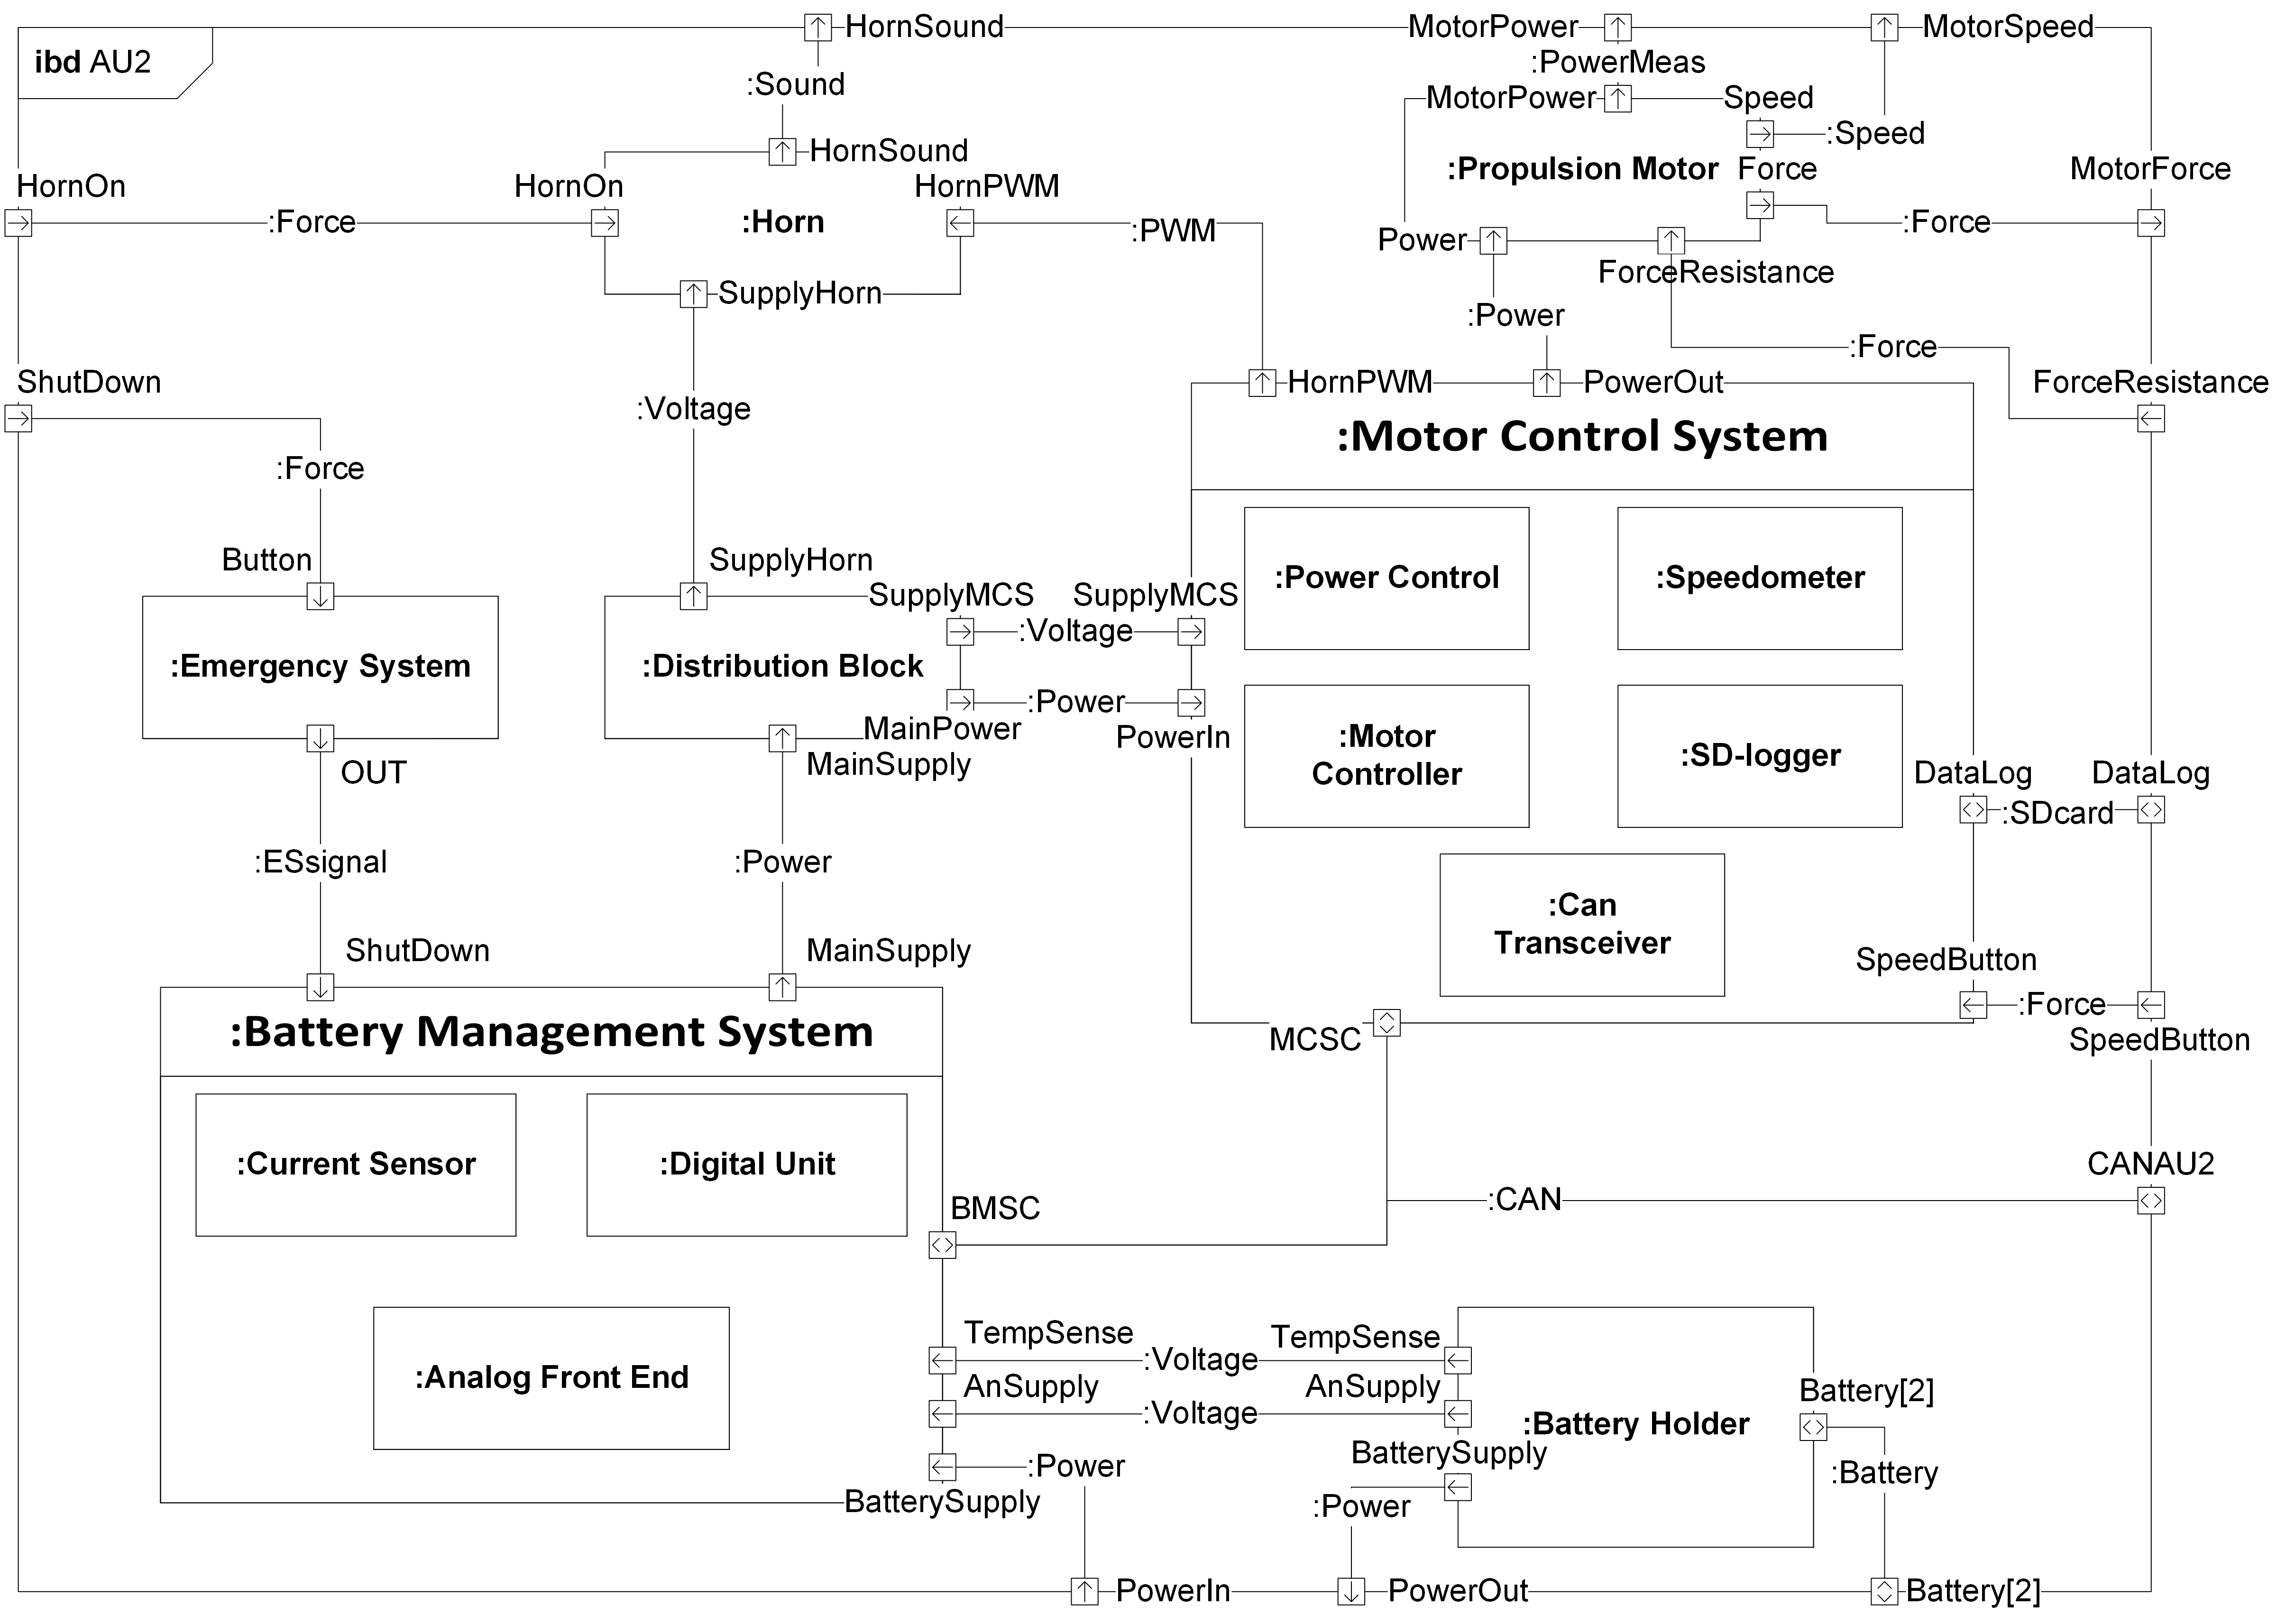
\includegraphics[width=1\linewidth]{Architecture/Diagrams/IBD_AU2}
	\caption{IBD for AU2}
	\label{fig:IBD}
\end{figure}

The supply-connection between the Distribution Block and the Motor Control System consists of two signals. This is represented by the bold connector. It should also be noted that both CAN-connections (BMSC and MCSC) are optional. They should only be connected when the user wants to read data from the BMS or the MCS.

The connection PowerMeas should only be used when AU2 is connected with Rolling Road for testing. This is represented by a dotted connector.